\section{Related Work}
\begin{figure}
  \centering
  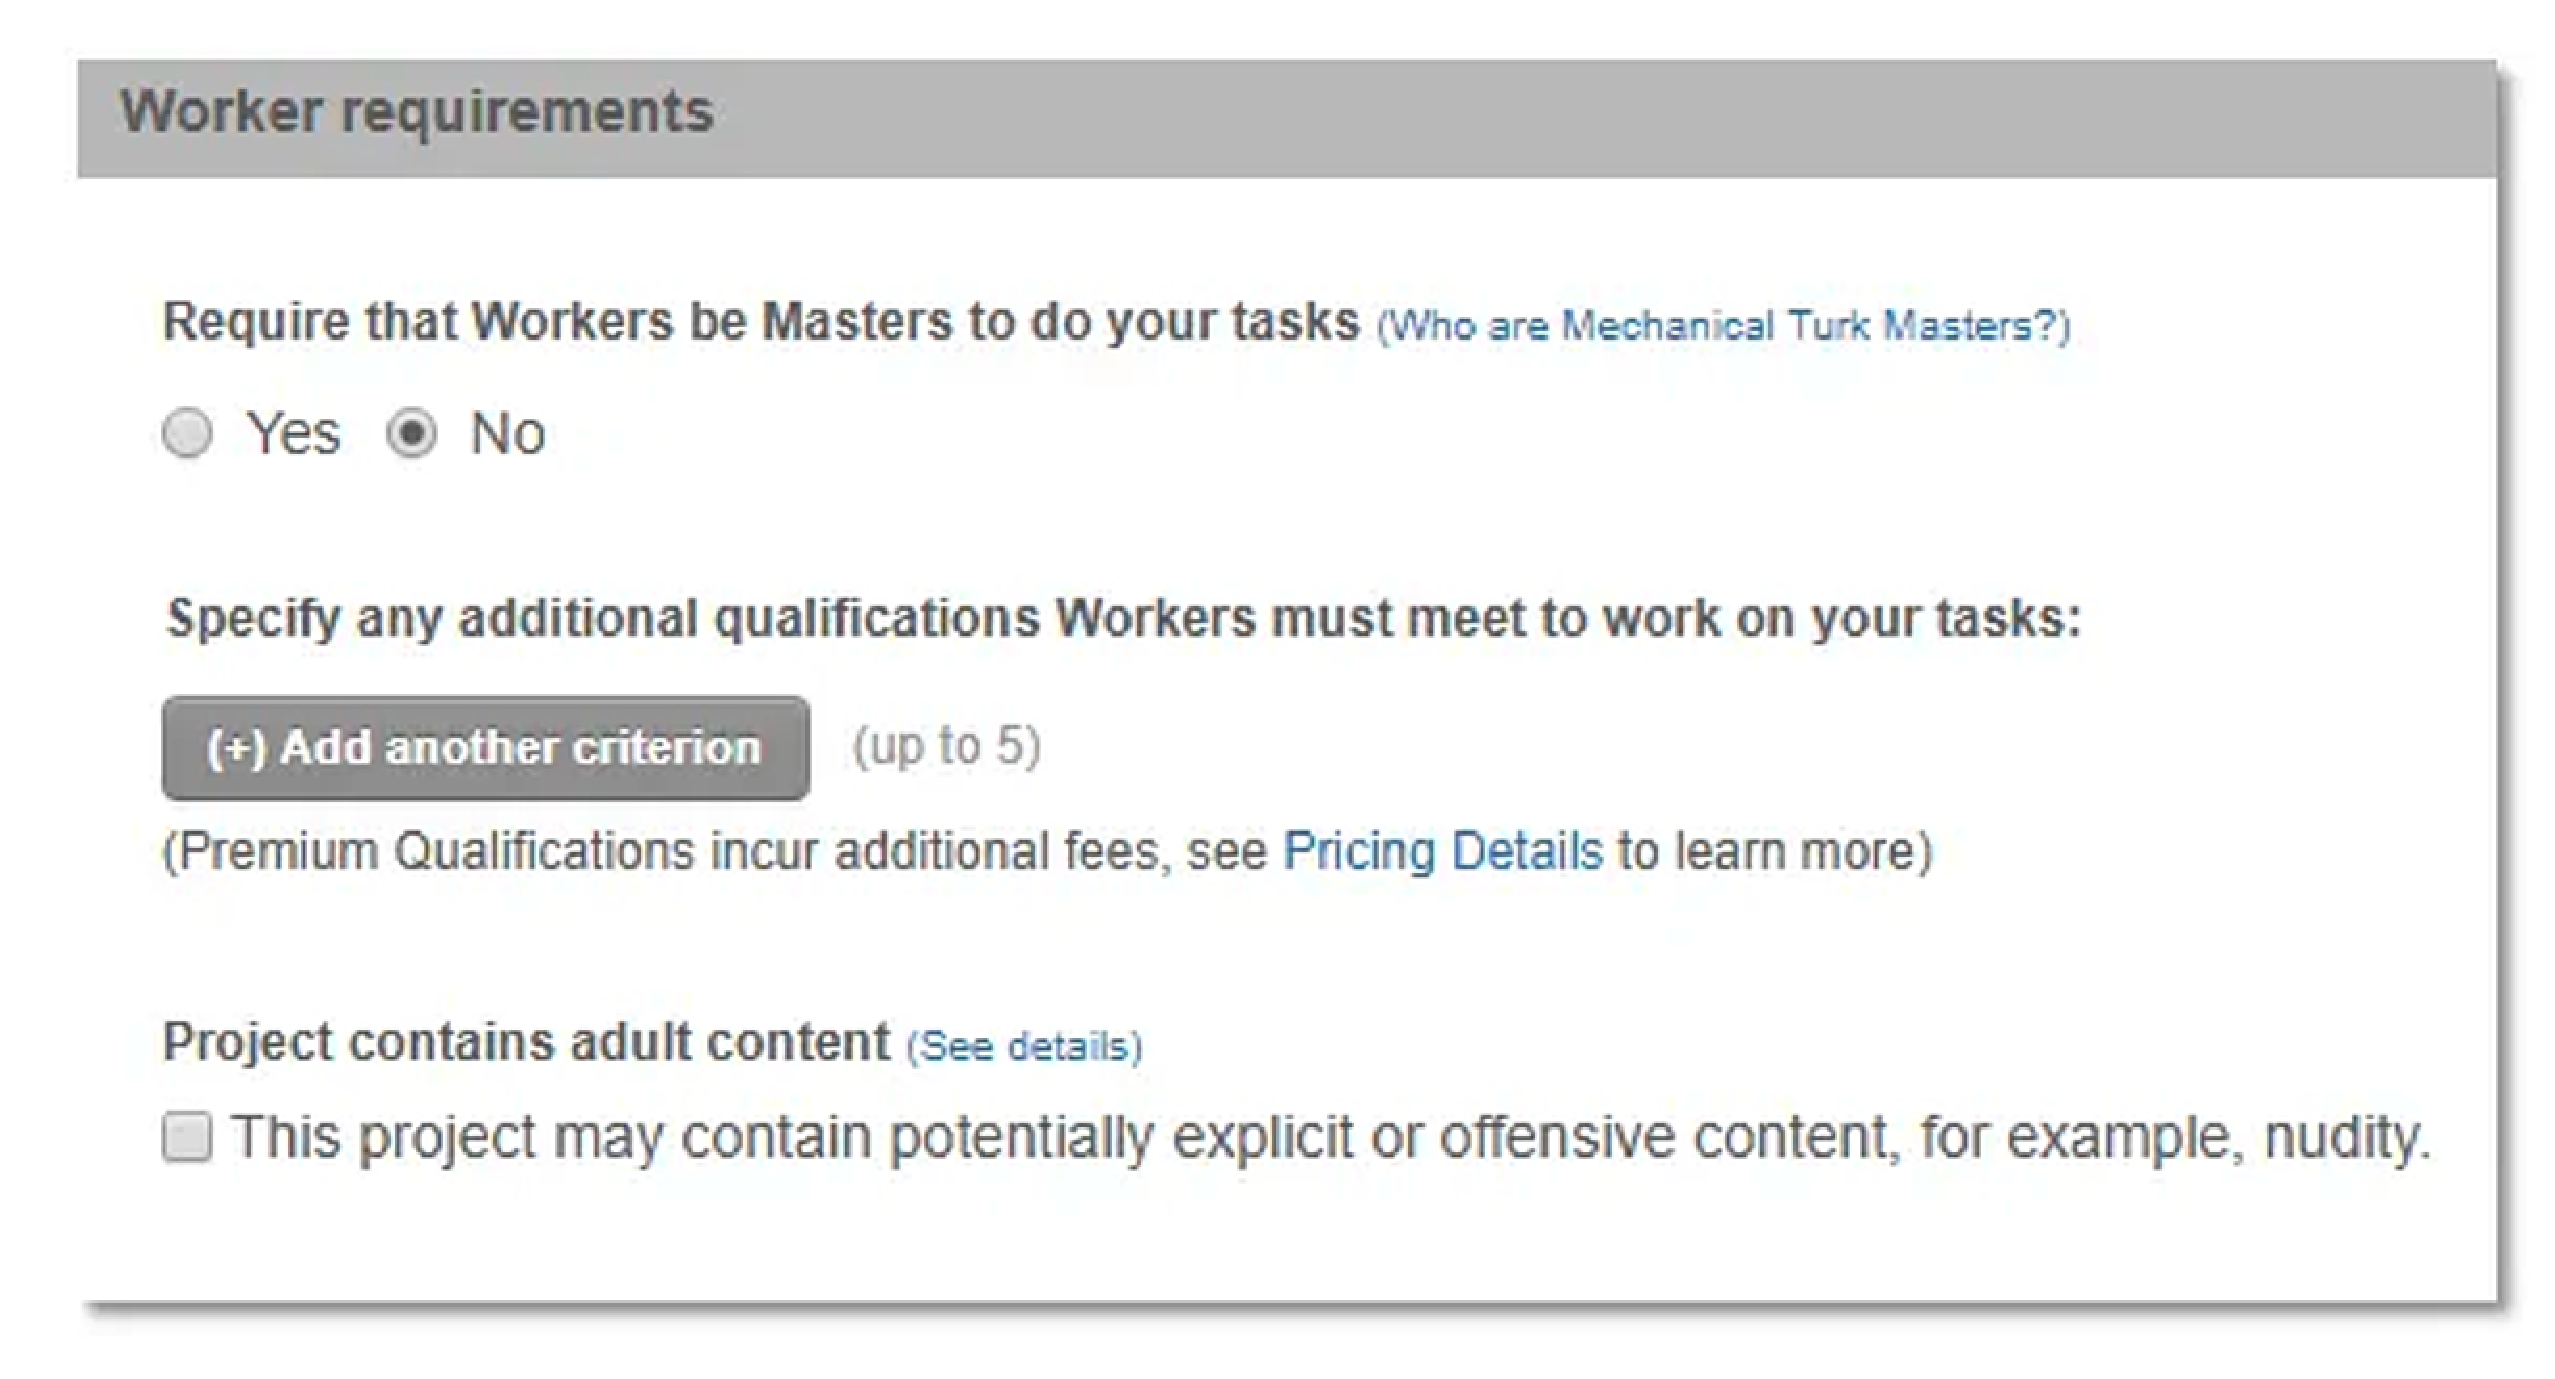
\includegraphics[width=0.6\linewidth]{figures/mturk_adult_qualification.pdf}
  \caption{MTurk’s adult content qualification requirement for screening workers.}
  \label{fig:mturk_adult}
\end{figure}


\begin{figure}
  \centering
  \begin{subfigure}[b]{0.48\linewidth}
    \centering
    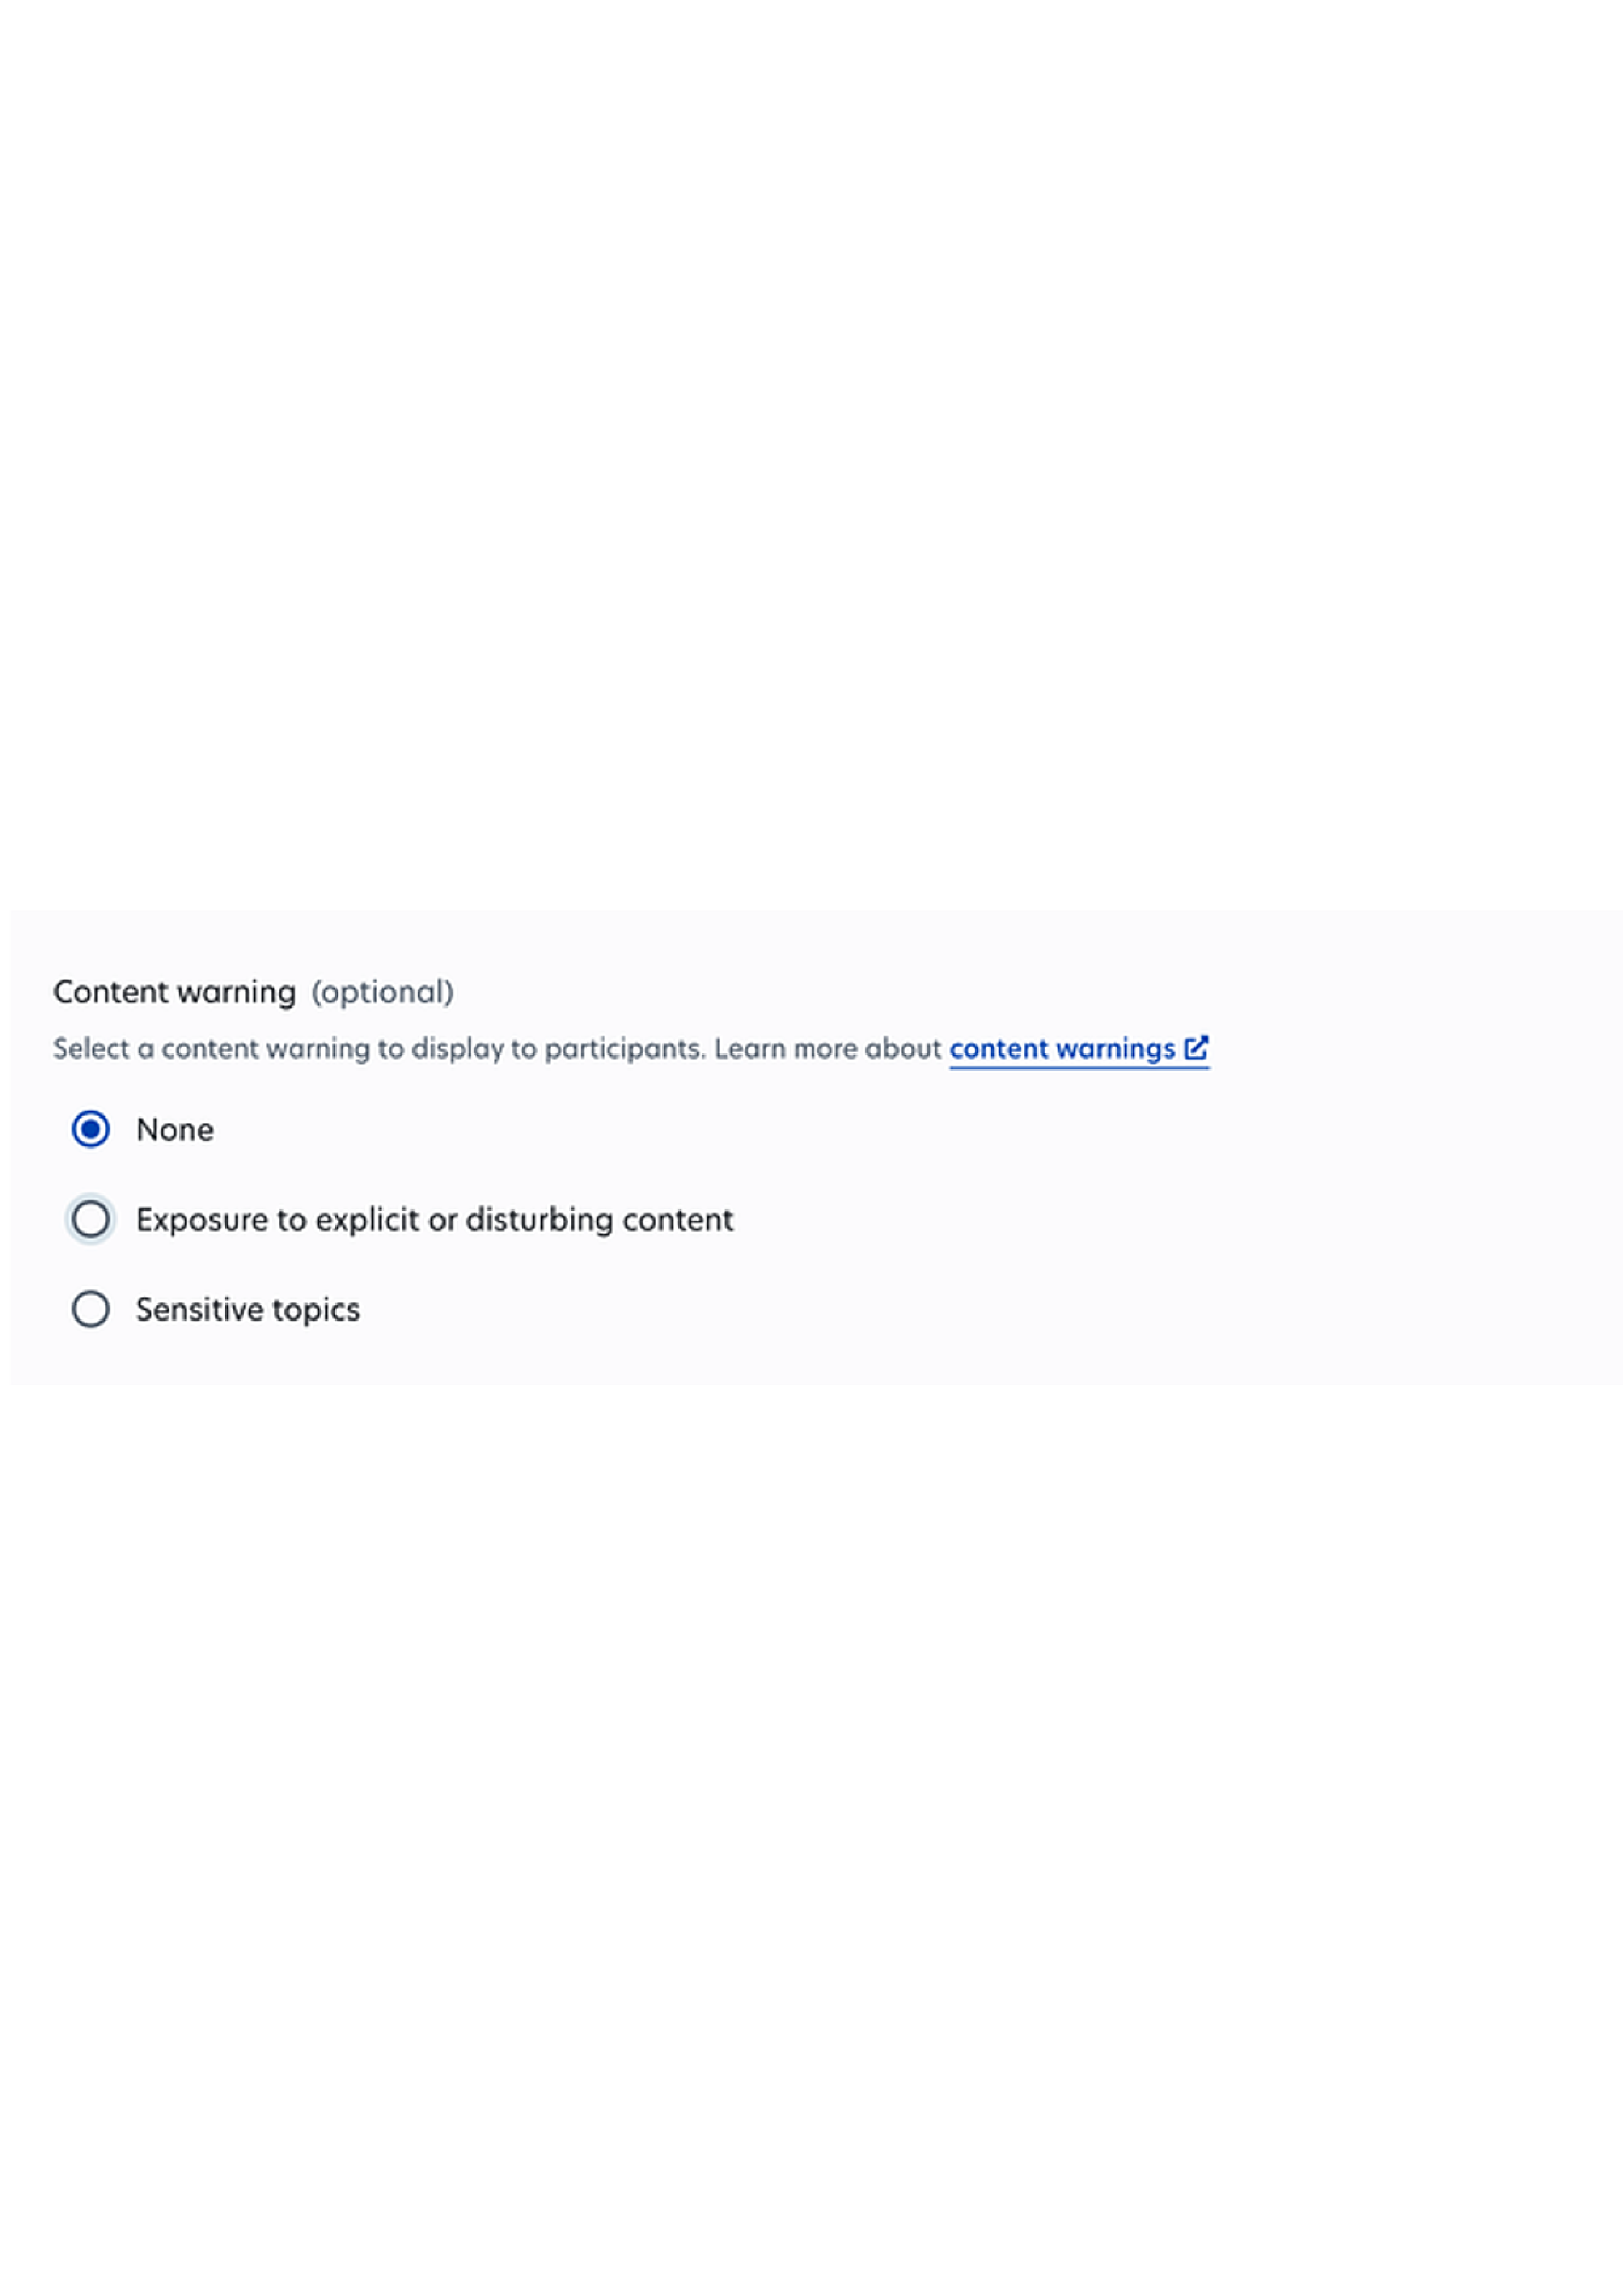
\includegraphics[width=\linewidth]{figures/prolific_zoomedin_binary.pdf}
    \caption{Close-up of the sensitive content warning presented to workers.}
    \label{fig:prolific_zoomed}
  \end{subfigure}
  \hfill
  \begin{subfigure}[b]{0.48\linewidth}
    \centering
    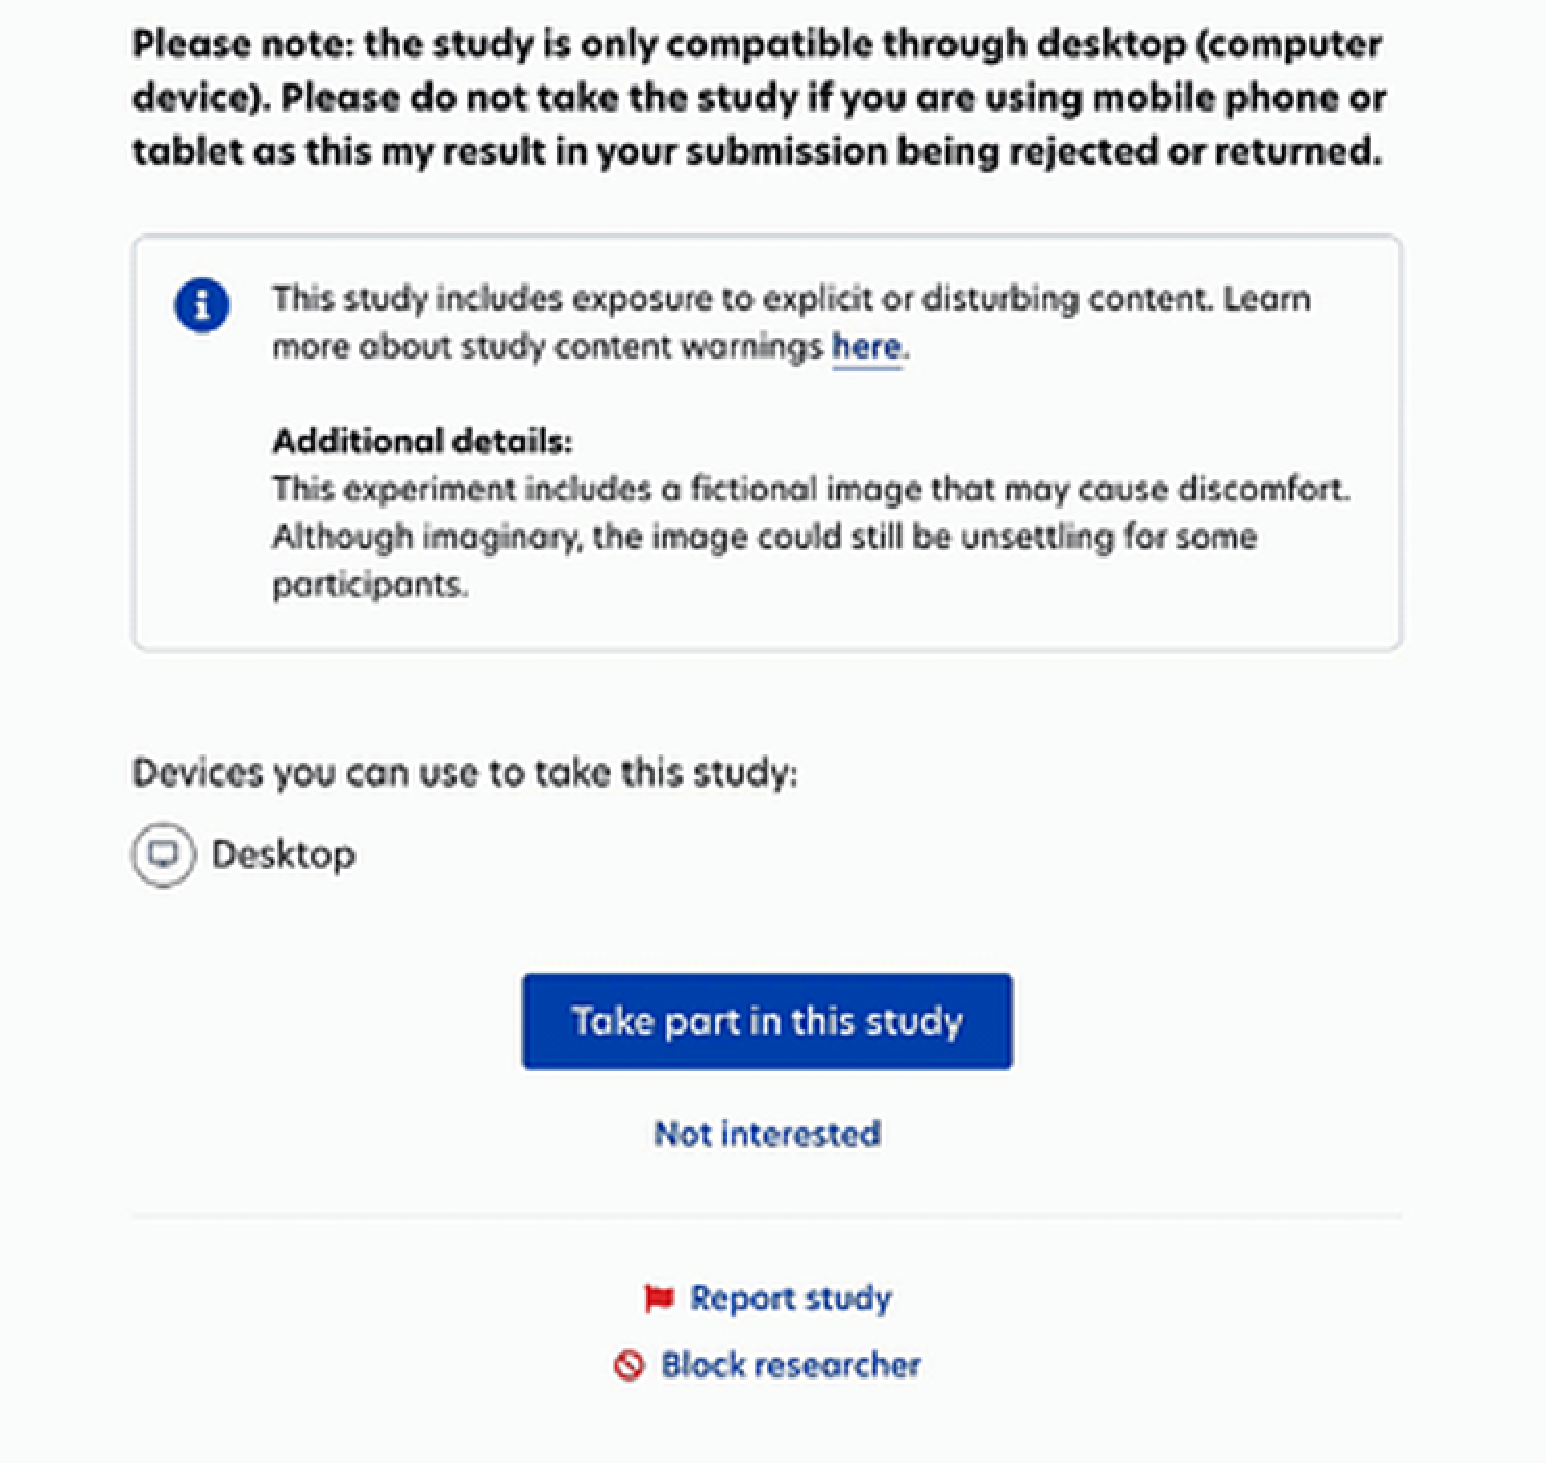
\includegraphics[width=\linewidth]{figures/prolific_worker_side_example.pdf}
    \caption{Worker-facing task list view with a sensitive content label.}
    \label{fig:prolific_worker}
  \end{subfigure}
  \caption{Prolific’s interface-level disclosure mechanisms from the worker perspective.}
  \label{fig:prolific_worker_pair}
\end{figure}

\begin{figure}
  \centering
  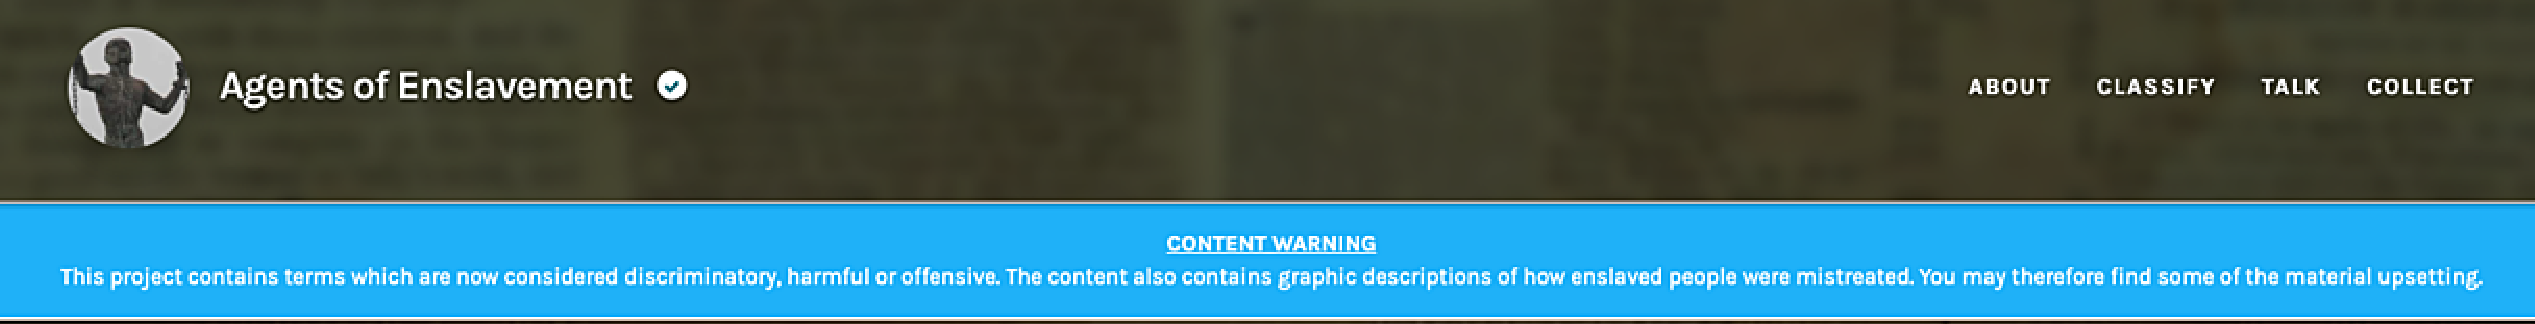
\includegraphics[width=\linewidth]{figures/warning_zooniverse.pdf}
  \caption{Task content warning from Zooniverse}
  \label{fig:zooniverse_removed}
\end{figure}

\begin{figure}
  \centering
  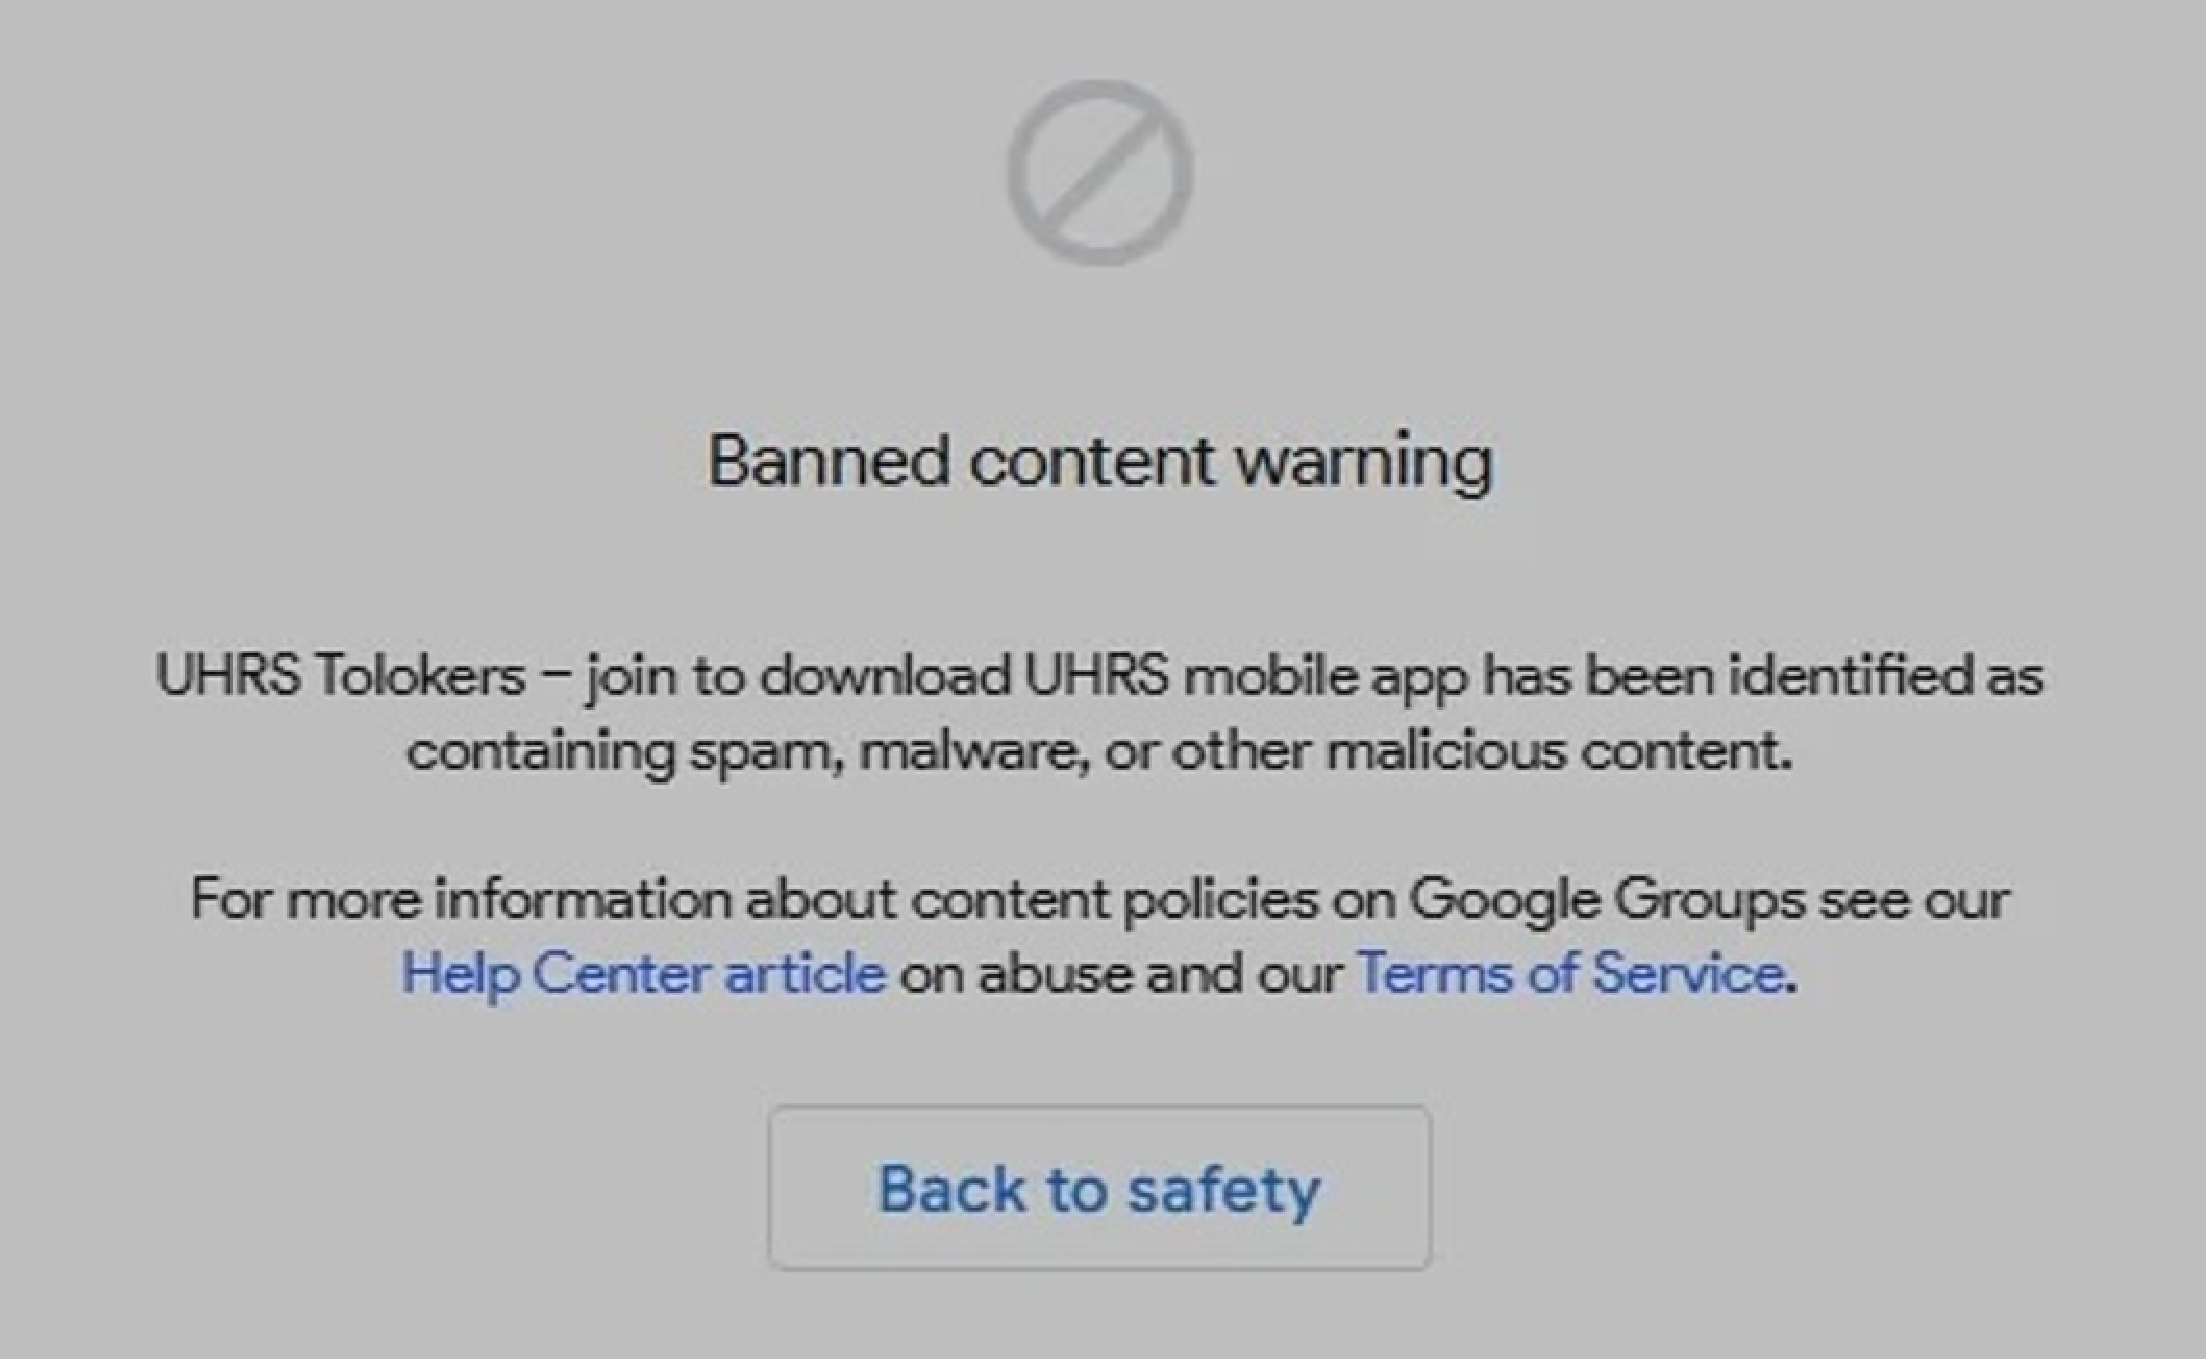
\includegraphics[width=0.7\linewidth]{figures/toloka_removed_task.pdf}
  \caption{Removed task page from Toloka, demonstrating limited access to past sensitive content.}
  \label{fig:toloka_removed}
\end{figure}


%\subsection{Risk Disclosure and Transparency in Crowdsourcing}
\subsection{Psychological and Well-being Risks of RAI Content Work} 
The rise of Responsible AI (RAI) initiatives draws new attention to the people behind the systems: workers who annotate, moderate, and evaluate AI content. These tasks -- collectively described as \textit{Responsible AI (RAI) content work} \cite{qian2025aura}, including annotation, moderation, and red teaming for model safety -- are critical to system performance and societal impact. Yet the labor remain largely invisible or undervalued ~\cite{gray2019ghost}. 

In particular, a growing body of research has documented the \textit{psychological and well-being risks} faced by these workers. Workers involved in those RAI content work routinely experience graphic or disturbing material with significant negative mental-health effects.  Studies show that prolonged exposure coupled with limited support contributes to burnout ~\cite{dosono2019moderation}, secondary trauma ~\cite{martinez2024secondary}, and PTSD ~\cite{steiger_psychological_2021, alemadi2024emotional, Michel2018ExContentMS, ruckenstein_re-humanizing_2020, Dwoskin_2019, arsht_2018_human}. More recent work replicates these findings, reporting that a large portion of content moderators exhibit moderate to severe psychological distress and low well-being \cite{Spence2025ContentModeratorMentalHealth}. Other research highlights broader harms, including privacy violations~\cite{pinchevski2023social, schopke-gonzalez_why_2022} and changes in workers’ personal beliefs and moral outlooks~\cite{newton_trauma_2019, Stackpole_2022, Douek_2021}.
%However, given the rapidly evolving nature of AI data work and limited investigation of employment contexts such as crowdsourcing, there is a pressing need to better understand the experiences, needs, and challenges of workers in these environments.

These well-being risks are compounded by the lack of support structures. While researchers are beginning to explore how organizations and individuals with decision-making power may support and address these psychological and well-being risks~\cite{qian2025aura, qian2025locating, steiger_psychological_2021, bharucha2023content}, most of this work has focused on full-time employees in formal moderation roles. Far less is known about how crowdworkers --- who perform similar tasks under more precarious conditions --- encounter and navigate these risks, which is the focus of this study.


\subsection{Risk Disclosure in Crowdsourcing Platform: A Multi-Stakeholder Challenge}
Although risk disclosure is recommended as a key practice to support worker well-being in RAI content work~\cite{bharucha2023content, qian2025aura}, it has primarily been discussed in the context of full-time employment and platform-based content moderation. This is a significant gap, as crowdworkers increasingly perform similar high-risk annotation and moderation tasks, often with little to no warning about potentially graphic or disturbing content, such as depictions of violence, self-harm, or abuse. These workers operate in task-based gig economies where formal protections like HR support or institutional mental health resources are typically absent~\cite{irani2013turkopticon, martin2014being, salehi2018ink, silberman2018responsible, toxtli2021quantifying, schlicher2021flexible}.

%be exposed to graphic or disturbing content, such as depictions of violence, self-harm, or abuse, without prior warning or support infrastructure. Unlike traditional employees, these workers often operate in task-based gig economies where formal HR policies or worker protections are absent~\cite{irani2013turkopticon, salehi2018ink, martin2014being, silberman2018responsible, toxtli2021quantifying, schlicher2021flexible}. As a result, the mechanisms and norms for disclosing potential harms in job postings or task instructions are highly variable.

%While prior literature has examined the psychological toll of content moderation specifically~\cite{spence2025content, alemadi2024emotional, steiger_psychological_2021}, which entails exposure to similarly harmful content as RAI content work \cite{qian2025aura, gillespie2025airedteamingsociotechnicalchallenge}, there is limited work describing how task-level risk information is communicated to annotators in crowdsourced settings. In this study, we investigate how risk should be disclosed in job ads and instructions for RAI content work tasks on crowdsourced work platforms. Our aim is to understand how task designers, workers, and platform representatives navigate risk disclosure mechanisms and the design tensions that emerge from tradeoffs shaping their disclosure decisions.
%\subsubsection{Risk Disclosure for Part-Time and Full-Time Jobs}

While prior HCI and CSCW work has extensively investigated the structural dimensions of crowdsourcing platforms, much of it has yet to address how well-being risks are communicated, managed, or shared. %  how crowdsourcing platforms are sites of recurring tension, where the balance among labor, automation, and governance is contested<CITES>. Platforms mediate a ``triadic relationship'' among workers, task designers, and the platform \cite{fieseler_unfairness_2019}. 
Foundational work by Irani et al. introduced Turkopticon, a system that surfaced worker–requester power asymmetries and challenged the opaque design of Amazon Mechanical Turk~\cite{irani2013turkopticon}. Following this, researchers have explored how platforms mediate relationships through design, algorithms, and incentives. Trade-offs between efficiency and fairness are deeply embedded in task workflows, reward structures, and rating systems~\cite{ho2015incentivizing}. Beyond facilitating labor, these systems act as sociotechnical infrastructures in which institutional values are deeply inscribed.
%Crowdsourcing acts as a sociotechnical infrastructure where values are encoded into design <CITES>.

From the worker's perspective, platform design can constrain or enable agency, but rarely centers on well-being. While crowdsourcing is often framed as flexible or empowering, studies show that this flexibility is unevenly distributed and often illusory~\cite{rechkemmer2022understanding, varanasi2022feeling, liang2021embracing}. Workers face well-documented challenges with task rejections~\cite{mcinnis2016taking}, opaque reputation mechanisms~\cite{saito2019turkscanner}, and emotional strain~\cite{flores2020challenges, martin2014being}, especially in tasks involving harmful or triggering content.

For task designers, the dominant focus is data quality, throughput, and consistency. However, recent work argues to re-examine how task designers might reflect on their interpretive and creative agency in shaping task content, instructions, and interaction dynamics~\cite{zheng2011task, bragg2018sprout, qian2025locating}. Studies have shown how task design choices --- including instruction clarity~\cite{wu2017confusing}, interface affordances~\cite{han2020crowd}, and incentive structures~\cite{ho2015incentivizing} --- can significantly influence worker outcomes. Calls for greater transparency in task designer identity and intention aim to help workers make more informed decisions and reduce asymmetries in trust and accountability~\cite{sutherland2018sharing, whiting2019fair, qian2025locating}.

At the platform level, governance practices shape how risk is managed, but often opaquely. Platforms mediate access to tasks, set rules, and enforce labor norms, but workers and task designers alike have limited visibility into these processes~\cite{toxtli2021quantifying, whiting2019fair, fieseler_unfairness_2019}. Algorithmic interventions, automated quality checks, and visibility constraints are not neutral; instead, they structure who gets to work, under what conditions, and with what recourse~\cite{gadiraju2017modus, rzeszotarski2012crowdscape}. While some platforms have introduced features aimed at promoting fairness and accountability~\cite{silberman2018responsible, whiting2019fair}, many continue to obscure institutional priorities behind claims of neutrality and scale~\cite{gray2016crowd, kingsley2015accounting}.

Yet despite these structural dynamics, little is known about how these stakeholders involved in RAI content work actually perceive, interpret, and implement risk disclosure in practice. Prior work has not examined how disclosure responsibilities are negotiated across roles, or what trade-offs shape real-world decisions. This paper addresses the gap by examining how task designers, workers, and platform representatives approach risk disclosure in crowdsourced RAI tasks. Through a multi-stakeholder investigation, we surface the tensions, frictions, and opportunities that shape disclosure practices, laying the groundwork for more transparent, protective, and equitable design.

\subsection{Risk Disclosure as a Design Challenge}
While academic and organizational discourse has increasingly underscored the importance of disclosing well-being risks in RAI content work, particularly for employed roles such as content moderators~\cite{bharucha2023content, qian2025locating}, less is known about how such efforts are operationalized in crowdsourcing contexts. %In particular, it remains unclear how workers and task designers perceive existing platform features intended to support disclosure, how those features function in practice, and what alternative designs should be explored.

%Task designers often lack structured guidance for implementing content warnings or consent flows in the task specification stage for RAI content work tasks~\cite{qian2025locating}. 

On the one hand, most crowdsourcing platforms offer limited, inconsistent, or opaque mechanisms for risk disclosure. % or ensuring their adoption when they do exist. One approach is allowing task designers to specify in different ways that their task contains sensitive content. 
Prolific, for example, provides a researcher-facing ``sensitive content'' toggle during study design (Figure \ref{fig:prolific_zoomed} along with an option to include additional information with keywords (see Figure \ref{fig:prolific_keywords}, along with guidelines to include warnings in task descriptions for both task designers ~\cite{ProlificResearcherSensitive2025, ProlificAPIContentWarning2025} and workers~\cite{prolific2025participant}. Another approach is to limit exposure based on age limits or other qualifications. Amazon Mechanical Turk (MTurk), for example, provides task designers with an ``adult content qualification'' requirement option in which only workers who have received this certification can see tasks with such content (see Figure \ref{fig:mturk_adult}). Research platforms such as Zooniverse and Tokola provide examples of task-level warnings (see Figure \ref{fig:zooniverse_removed} and Figure \ref{fig:toloka_removed}), but these remain inconsistent in format and enforcement.
%Platforms such as DataAnnotation, Remotasks, and SurgeAI, lock their interfaces behind employment verification systems, and publicly available information about their risk disclosure process is scarce. Platforms used for crowdsourced research, such as Zooniverse and Tokola, have documented similar types of warnings for tasks (see Figure \ref{fig:zooniverse_removed}).  At the surface level we see a lack of consensus across platforms around how risk disclosure should be supported within crowdsourcing infrastructures.
Beyond disclosure options, platform-level governance also varies significantly. %Platforms have the power to moderate or enforce risk disclosures. There is limited publicly available documentation, however, on how platforms make decisions on what tasks or content are permitted. 
For example, Prolific allows workers to report tasks for review and potential removal, and anecdotal evidence suggests platforms like Toloka have occasionally removed tasks after worker complaints (Figure~\ref{fig:toloka_removed}). However, such interventions appear to be the exception rather than the norm.

On the other hand, past work on content warnings on consumer-facing platforms offers important lessons for designing risk disclosures for RAI work. Social media platforms such as Tumblr, Twitter (now X), Instagram, and TikTok have implemented content warnings to protect users from potentially distressing material, ranging from textual tags like \#tw to automated overlays that blur graphic images. These systems aim to support informed consent, reduce harm, and signal sensitivity to trauma~\cite{Zhang2024PerceptionsTriggerWarnings, vit2025use}. However, their application is highly variable and their effectiveness remains contested. Empirical studies show that while users generally appreciate warnings in principle, concerns persist about inconsistent enforcement, insufficient granularity, and unclear rationale~\cite{charles2022typology, bridgland2024meta, bell2025warning}. Some warnings may even increase anticipatory anxiety, especially among individuals with lived experience of trauma~\cite{sharevski2022meaningful}. These limitations highlight the complexity of operationalizing harm reduction at scale and suggest that risk disclosure is not simply a matter of adding labels, but requires careful design attuned to user needs, platform affordances, and sociocultural context.

More importantly, the context of crowdsourced RAI work differs in important ways. Unlike social media users, who encounter warnings during voluntary content consumption, crowdworkers engage with potentially harmful material as part of paid, high-throughput tasks. As such, risk disclosure in this domain intersects with distinct incentives -- such as performance expectations, compensation structures, and data quality requirements -- that reshape the meaning of consent, exposure, and protection. These differences raise critical questions about how content warning strategies must be re-imagined for labor systems, not simply adapted from consumer platforms.

In this study, we build on these insights to examine how risk disclosure is approached, interpreted, and contested in the context of crowdsourced RAI content work. We frame risk disclosure not as a compliance checkbox or content tag, but as a complex design challenge that must account for divergent stakeholder needs, uneven power relations, and structural gaps in responsibility and support.

%Overall, platform-level features for risk disclosure are inconsistent, unreliably enforced, and often rely on the initiative of individual task designers. Without formalized mechanisms for validation or enforcement, responsibility for ethical disclosure is effectively decentralized. This ambiguity raises critical questions about accountability and reveals how existing systems prioritize flexibility and throughput over standardized support. In this study, we examine how risk disclosure dynamics are navigated in practice by workers, task designers, and platforms alike and how current approaches reflect broader tensions between different stakeholder. %We conceptualize risk disclosure as a design space defined by timing of disclosure before or during or after a task, scope and granularity of information, control over gating and opt out, visibility to stakeholders, validation of claims, and enforcement mechanisms.


% Transparency tools such as model cards, datasheets and crowdworksheets document model behavior and data provenance but seldom address worker well-being; meanwhile, research on trigger and content warnings reveals the complexities of communicating risks to users.  Computational efforts aim to automatically assign trigger warnings to social media posts and fan-fiction \todo{citations}, but performance remains modest and the taxonomy of warnings is contested~\cite{Wiegmann2023Trigger}.  Bridgland et al.’s meta-analysis of trigger-warning experiments finds that warnings do not reduce distress and may increase anticipatory anxiety~\cite{Bridgland2024Meta}, highlighting the lack of consensus about their effectiveness.  Diaz et al.’s CrowdWorkSheets framework calls for documenting annotator demographics and decision points in data collection~\cite{Diaz2022CrowdWorkSheets}, while Turri et al.\ argue that existing transparency efforts focus on downstream users and overlook the needs of data creators and moderators~\cite{Turri2024Transparency}.  These findings support our claim that current tools fall short in communicating risks to workers and that empirically grounded disclosure mechanisms are needed.





%\subsection{Lessons from Content Warnings on Social Media Platforms}
%\todo{Add a brief review of research on warnings from human factors? like pre-internet research}
% from laura
% https://www.sciencedirect.com/science/article/pii/S0003687002000091?casa_token=PRWc3Ycbrj0AAAAA:pETsBivTstXdlz9obPRdNyFX8RKeZktc-OR7nvAxqvO1_kt0wJAwOS8lTglhAqzZoTAaXfsFdg#BIB99
% https://www.sciencedirect.com/science/article/pii/S0003687002000091?casa_token=PRWc3Ycbrj0AAAAA:pETsBivTstXdlz9obPRdNyFX8RKeZktc-OR7nvAxqvO1_kt0wJAwOS8lTglhAqzZoTAaXfsFdg
%Content warnings on social media platforms are an example of a platform-level intervention for communicating content risk. Digital content and trigger warnings (TWs/CWs) were originally developed by social media platforms as a mechanism to give users greater control over their exposure to distressing content. Platforms such as Tumblr, Twitter (now X), Instagram, and TikTok have increasingly relied on warnings to label content related to potentially disturbing topics such as self-harm, suicide, eating disorders, more. These warnings serve multiple purposes: protecting users’ psychological well-being, signaling platform sensitivity to trauma, and minimizing liability through proactive disclosure~\cite{Zhang2024PerceptionsTriggerWarnings, vit2025use}. Although these content warning systems represent risk communication design work, they've primarily been implemented in consumer-facing contexts rather than labor platforms.

%Content warnings appear in varied forms~\cite{charles2022typology}. Some are user-applied tags or hashtags (e.g., \#tw, \#cw), while others are system-generated overlays that blur images or restrict content with interstitial warnings such as ``sensitive content ahead.'' Warnings are often differentiated by modality: graphic video content might receive stricter AI-driven flags, whereas textual descriptions rely more on user discretion. The rationale behind these warnings can differ: some aim to reduce harm, others to promote informed consent or foster a respectful discourse environment~\cite{gomes2024problematizing}. This diversity reflects both the flexibility and inconsistency in how platforms define risk and empower users, raising questions about how such designs might or might not translate into the labor context.

% should probably add a figure somewhere here
%Although widely adopted, existing content warning systems are not without limitations. Despite their intentions, content warning systems remain contested~\cite{sharevski2022meaningful, vitak_beyond_2016}. Interviews with social media users show a broad consensus that warnings are helpful in principle, yet concerns persist around inconsistent application, limited nuance, and unclear guidelines for use~\cite{Zhang2024PerceptionsTriggerWarnings}. Some users expect systems to preemptively shield them from trauma, while others see warnings as overly cautious or stifling to expression. Empirical studies suggest that warnings often do little to reduce emotional distress and may even increase anticipatory anxiety, especially among individuals with relevant lived experience~\cite{bridgland2024meta, bell2025warning}. In practice, it remains a challenge to strike a balance between over-warning and under-warning in these systems, with the burden frequently falling on creators to self-disclose in the absence of clear platform guidance~\cite{vit2025use}. These shortcomings highlight the challenges of operationalizing harm reduction at scale, insights that are highly relevant to understanding risk disclosure mechanisms in crowdsourced labor environments.

% Content moderation policies vary significantly across social media platforms, and enforcement remains opaque and inconsistent~\cite{gomes2024problematizing, gibbs2015facebook}. Though the U.S. Surgeon General has called for warning labels to protect youth mental health (i.e., analogous to tobacco packaging warnings) these proposals remain politically and legally contested~\cite{murthy2024surgeon}. Such tensions between user expectations and platform enforcement underscore the difficulty of balancing protection, autonomy, and expression, dynamics that are equally salient in worker-facing systems. 

%Taken together, content warnings represent a growing, if imperfect, strategy for risk disclosure in digital environments. Yet despite their increasing adoption in consumer-facing media, few analogues exist for informing crowdworkers of potentially distressing material. Understanding how labor-specific practices diverge from social media conventions is critical for designing effective and equitable disclosure mechanisms in AI data pipelines.

%Unlike social media users, who encounter warnings as part of their content consumption experience, crowdworkers engage with potentially harmful material in a professionalized, task-based context. As such, decisions about risk disclosure intersect with different incentives and values, such as task performance, compensation, data quality, and organizational responsibility. By studying disclosure practices in this distinct setting, we extend existing research on digital risk communication and examine how concepts like user agency, transparency, and consent play out in the behind-the-scenes labor of AI safety. Importantly, our work aims to critically examine how elements of risk communication may be meaningful within crowdsourcing workflows.


%HCI research has long documented how crowdsourcing platforms are sites of recurring tension, where the balance among labor, automation, and governance is contested<CITES>. Platforms mediate a ``triadic relationship'' among workers, task designers, and the platform \cite{fieseler_unfairness_2019}. Foundational work by Irani et al. introduced Turkopticon, a system that surfaced worker–requester power asymmetries and challenged the opaque design of Amazon Mechanical Turk~\cite{irani2016turkopticon}. Following this, researchers have explored how platforms mediate relationships through design, algorithms, and incentives. Trade-offs between efficiency and fairness are deeply embedded in task workflows, reward structures, and rating systems~\cite{ho2015incentivizing, BLANK, BLANK}. Crowdsourcing acts as a sociotechnical infrastructure where values are encoded into design <CITES>.

%A large body of prior research has examined how, from the perspective of the worker, platform design constrains or enables agency, autonomy, and well-being. While crowdsourcing offers flexibility, studies reveal how this flexibility is often unevenly distributed, uncertain, or illusory in practice~\cite{rechkemmer2022understanding, varanasi2022feeling, liang2021embracing}. Workers face challenges with task rejection mechanisms~\cite{mcinnis2016taking}, reputation~\cite{saito2019turkscanner}, and emotional risks ~\cite{martin2014bein, flores2020challenges} that are often invisible to requesters or platform administrators~\cite{flores2020challenges, martin2014being}. 

%Requesters---whom we refer to here as task designers---often prioritize data quality, consistency, and throughput. Prior research has advocated for this shift in framing of the role of individuals designing and posting RAI content work tasks because the term ``requester'' may suggest a transactional role centered on task submission and payment, whereas ``task designer'' foregrounds the creative and interpretive decisions that shape task content, instructions, and interaction flow~\cite{zheng2011task, bragg2018sprout, alagarai2014cognitively, allen2018design, qian2025locating}. Additionally, prior work has explored how task designers can vary incentives to elicit more accurate or creative responses~\cite{ho2015incentivizing} and how task instructions and interfaces influence labor outcomes~\cite{wu2017confusing, han2020crowd}. Some studies have advocated for greater transparency in task designer identity, goals, and decision-making processes, particularly to help workers make informed choices and build trust~\cite{sutherland2018sharing, whiting2019fair, qian2025locating}.

%At the platform level, prior research has examined how governance practices structure interactions and outcomes for both workers and task designers~\cite{toxtli2021quantifying, whiting2019fair, fieseler_unfairness_2019}. Platforms can mediate access to work, enforce rules, arbitrate disputes, and set the terms under which labor occurs. Algorithmic interventions, data visibility constraints, and automated quality controls are not neutral mechanisms but embedded forms of power that affect how labor is valued and by whom~\cite{gadiraju2017modus, rzeszotarski2012crowdscape}. While some platforms have introduced features to increase fairness or accountability~\cite{whiting2019fair, silberman2018responsible}, others have maintained opaque infrastructures that obscure institutional priorities. Crowdsourcing platforms act as powerful intermediaries whose governance models reflect complex trade-offs between stakeholder needs, regulatory risk, and commercial interests~\cite{gray2016crowd, kingsley2015accounting}.
%Crowdsourcing ecosystems are deeply entangled with social, economic, and political concerns. Designing for such systems requires more than recognizing trade-offs, it requires actively negotiating them, building tools and frameworks that make underlying tensions visible and open to contestation.

% , and how task designer behaviors contribute to broader patterns of fairness, exclusion, or epistemic inequality~\cite{BLANK}

\subsection{Co-Designing Risk Disclosure Across Stakeholders}
Given the socio-technical complexity of risk disclosure in crowdsourced RAI work, we adopt a co-design approach grounded in the belief that design decisions should not be made solely by researchers. Rather, they should be informed by those most affected by the system: in this case, task designers, crowd workers, and platform representatives. By foregrounding these perspectives, co-design allows us to surface tensions that may remain hidden in researcher-led or single-stakeholder-oriented design processes.
Co-design is often associated with participatory and equitable research practices~\cite{muller_participatory_nodate} and has proven especially valuable in navigating contested design spaces such as gig work and freelance work \cite{huang2024design, hsieh_designing_2023}. In these contexts, co-design serves not only to generate design ideas but to redistribute power in the research process, allowing participants to shape the framing of problems, not just react to solutions.

Despite growing recognition of the risks embedded in RAI content work, few studies have examined how these risks might be communicated or who should bear the responsibility of disclosure. To our knowledge, this research is among the first attempts to apply co-design to examine risk disclosure in the crowdsourcing context, with direct input from all three stakeholder groups. Our approach builds on prior calls to design for multi-stakeholder participation  \cite{vines2013configuring}, recognizing that risk disclosure is not a simple matter of transparency but an ongoing negotiation of accountability, agency, and institutional power. %stakeholder needs.




% Transparency tools such as model cards, datasheets and crowdworksheets document model behavior and data provenance but seldom address worker well-being; meanwhile, research on trigger and content warnings reveals the complexities of communicating risks to users.  Computational efforts aim to automatically assign trigger warnings to social media posts and fan-fiction \todo{citations}, but performance remains modest and the taxonomy of warnings is contested~\cite{Wiegmann2023Trigger}.  Bridgland et al.’s meta-analysis of trigger-warning experiments finds that warnings do not reduce distress and may increase anticipatory anxiety~\cite{Bridgland2024Meta}, highlighting the lack of consensus about their effectiveness.  Diaz et al.’s CrowdWorkSheets framework calls for documenting annotator demographics and decision points in data collection~\cite{Diaz2022CrowdWorkSheets}, while Turri et al.\ argue that existing transparency efforts focus on downstream users and overlook the needs of data creators and moderators~\cite{Turri2024Transparency}.  These findings support our claim that current tools fall short in communicating risks to workers and that empirically grounded disclosure mechanisms are needed.
